%!TEX root = main.tex
% \begin{figure}[htb]
% \begin{center}
% %optional pour enlever un peu d'espace blanc de votre silhouette
% %\vspace{-.3cm}
%  %\includegraphics[keepaspectratio,width=0.5\textwidth]{fig/nomde}
% % analoog
% %\vspace{-0.6cm}
%  % \caption{ici un logo}
%  % \label{fig:ruglogo}
% %analoog
% %\vspace{-.6cm}
% \end{center}
% \end{figure}

% Utilisation du template
% \cite(reference à citer)
% \ref(figure à référencer)

\chapter{Axes de Recherches : WGAN}

\paragraph*{} Avec les différents résultats obtenus par nos premiers GAN, nous avons pu tirer, entre autres, deux conclusions importantes. Le GAN manque cruellement de stabilité (par exemple un petit changement de paramètre l'empêche de converger correctement) et de métriques pertinentes, c'est à dire que les scores des générateurs et des discriminateurs n'ont pas d'interprétations en termes de progrès de la qualité d'image perçue.\\
Les chercheurs se sont beaucoup attardés depuis 2016 sur la première question, en comparant par exemple les différents optimiseurs possible \cite{opimiser}, le deuxième point est lui moins souvent abordés. \\
L'article de 2017 Wasserstein GAN \cite{wgan} propose une méthode qui, en s'éloignant légèrement de la philosophie original du papier de Goodfellow \cite{Goodfellow-et-al-2016}, tente d'apporter une réponse à ces deux questions, avec, en particulier, une métrique pertinente.

\section{Problématique de la descente de gradient simultanée}

L'article de Goodfellow semble démontrer la convergence du système GAN, cependant la mise en œuvre montre que cette convergence n'est pas aussi évidente à obtenir. En effet, il semblerait que la stratégie de descente de gradient de l'algorithme de GAN ne permette pas d'assurer cette convergence. Le blog inFERENCe \cite{conservative-field} décrit une partie du problème en se basant sur l'article The Numerics of GANs \cite{numerics-gan}.

Ces articles montrent que la descente de gradient simultanée n'est pas simplement une double descente de gradient, mais une descente de gradient dans un champ vectoriel. l'algorithme de GAN effectue l'optimisation suivante : 
\[x_{t+1} \leftarrow x_t + h v(x_t) \text{ avec } v(x) = \left(\begin{matrix}\frac{\partial}{\partial\theta}f(\theta, \phi)\\\frac{\partial}{\partial\phi}g(\theta, \phi)\end{matrix}\right).\]

$f$ et $g$ étant respectivement les fonctions de coût du Discriminateur et du Générateur. Cependant on constate 2 problèmes. D'une part, l'algorithme basé sur la théorie des jeux, qui consiste à faire "jouer" tour à tour le Discriminateur et le Générateur pour optimiser ses paramètres ne consiste qu'en une approximation de la simultanéité de la descente. D'autre part, il n'y a aucune preuve que le champ vectoriel $x$ dans lequel l'on se déplace possède des propriétés conservatives. En particulier, rien ne garantit que le rotationnel soit nul, ce qui implique que la descente de gradient ne soit pas garantie d'aller vers un minimum, même local (Figure : \ref{fig:vector_field})!

\begin{figure}[ht!]
  \centering
    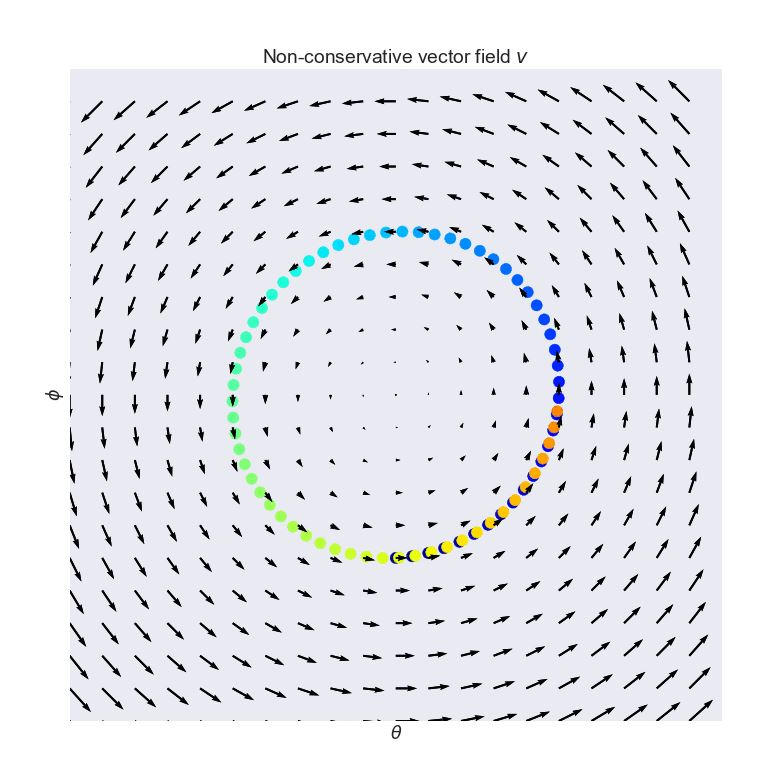
\includegraphics[width=10cm]{fig/vector_field}
    \caption{champ vectoriel non conservatif : exemple de descente de gradient}
    \label{fig:vector_field}
\end{figure}

On est donc à la recherche d'une autre approche qui contournerait ce problème.



\section{L'approche Wasserstein GAN}

Le papier Wasserstein GAN \cite{arjovsky_wasserstein_2017}, propose une autre approche que celle de la théorie des jeux.

Il s'agit de calculer une divergence entre distributions afin de se servir de cette métrique pour faire l'apprentissage de l'une sur l'autre. Au premier abord, cette approche ne semble pas si éloignée de l'approche de Goodfellow, mais elle en est sensiblement différente. Dans l'approche précédente, on tente de minimiser la divergence entre deux distributions par un algorithme utilisant 2 réseaux de neurones. Cependant, nous n'avons jamais accès à cette divergence (que l'on utilise des fonctions d'erreur pour approcher la KL-divergence ou une autre), et comme nous l'avons montré précédemment, la convergence n'est pas réellement assurée. 

L'idée du papier Wasserstein GAN est de calculer explicitement une divergence entre deux ensembles. Cela n'est pas une question simple, comme nous avons pu le voir au chapitre 1. En effet, nous n'avons généralement pas accès à la distribution $p_{\text{réel}}$ mais uniquement à un échantillon tiré de cette distribution. \\ Cependant il apparait possible de calculer une divergence entre deux ensembles à l'aide des réseaux de neurones. Cela est possible en tout cas avec la divergence de Wasserstein, comme le montre ce papier, nous allons revenir sur les étapes de raisonnements.

L'objectif est de rapprocher 2 distributions en utilisant la métrique de Wasserstein à l'ordre 1. Celle-ci s'écrit :
\[
W(\mathbb{P}_r, \mathbb{P}_g)= \underset{\gamma \in (\mathbb{P}_r, \mathbb{P}_g)}{\text{inf}} \mathbb{E}_{(x,y)\sim\gamma} \left[ ||x-y||\right]
\]
On peut la nommer également distance Earth-Mover, c'est à dire distance du déplacement de terre. En effet cette métrique calcule l'effort à faire pour passer d'une distribution à l'autre (Figure : \ref{fig:E-M_distance}). Par exemple, si l'on a deux terrains contenant des tas de terre, la hauteur de terre en un point représente la densité de probabilité à cette endroit, le volume complet de terre étant le même (cela représente l'intégrale sur le terrain), alors la distance EM entre les deux terrains est l'effort minimal que l'on peut faire pour déplacer la terre de l'un des terrains pour le faire ressembler à l'autre. Il y a une infinité de façons de déplacer la terre, avec des efforts différents. La distance de Wasserstein est le coût en utilisant le plan de transport optimal. Cela se traduit également en termes de probabilités jointes, pour une approche plus mathématique. 

\begin{figure}[ht!]
  \centering
    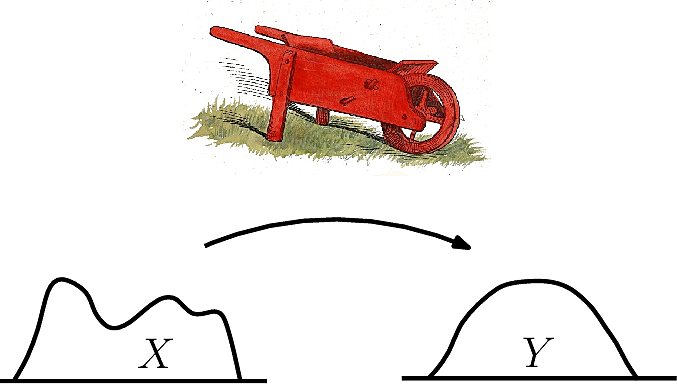
\includegraphics[width=10cm]{fig/Earth_mover_distance}
    \caption{Illustration de la divergence Earth-Mover}
    \label{fig:E-M_distance}
\end{figure}


L'idée d'utiliser cette divergence de Wasserstein provient des propriétés mathématiques qui lui sont propre. Cette divergence est théoriquement plus pertinente pour l'apprentissage des GANs. Le détail se trouve dans ce papier, mais cela se peut se résumer ainsi : Wassertein donne plus d'informations que la KL-Divergence et ses dérivées (Jensen-Shannon, etc) en étant, entre autres, bien définie lorsque les supports de distribution sont disjoints et en étant moins souvent constante, avec donc des gradients non nuls et plus adaptés à l'apprentissage.

On ne peut toujours pas se servir de cette divergence, mais un théorème (la dualité Kantorovich-Rubinstein \cite{optimal-transport}) permet d'obtenir une nouvelle forme de cette divergence :
\[
W(\mathbb{P}_r, \mathbb{P}_g) = \underset{||f||_L<1}{\text{sup}}\mathbb{E}_{x\sim\mathbb{P}_r}\left[f(x)\right] - \mathbb{E}_{x\sim\mathbb{P}_g}\left[f(x)\right]
\]
Vous pouvez en voir une preuve simplifiée sur le blog de Vincent Hermann \cite{preuve-wgan}.
On se retrouve alors à calculer un sup sur un ensemble de fonctions (les fonctions 1-Lipschitziennes), et cela est pratique car c'est justement ce que permet de faire un réseau de neurones : Simuler des fonctions que l'on optimise par rapport à un paramètre ! On construit un réseau qui joue le rôle des fonctions f, on a donc des paramètres $W$ à optimiser pour trouver la valeur maximum. Il ne reste qu'à s'assurer que les réseaux de neurones peuvent garantir le caractère 1-Lipschitzien.

Une méthode pour s'assurer de cette propriété est de restreindre les poids dans un intervalle [-c, c] (on parle de weight-clipping). Cependant on obtient un caractère K-Lipschitzien, avec un K inconnu. (En terme de preuve, il suffit de voir que des matrices avec ses propriétés sont toutes K-Lipschitziennes avec un même K.) Cela nous assure que l'on peut calculer non pas $W(\mathbb{P}_r, \mathbb{P}_g)$ mais $K*W(\mathbb{P}_r, \mathbb{P}_g)$, mais le K étant fixe tout au long de l'apprentissage cela reste une métrique pertinente. 

Nous avons donc la possibilité avec un réseau de neurones de calculer la métrique de Wasserstein et nous allons pouvoir nous en servir pour l'apprentissage d'un générateur.

\section{Mise en œuvre}

Fort de cette métrique que l'on peut calculer, nous allons pouvoir mettre en place un algorithme d'apprentissage pour la génération d'image.

Tout d'abord, nous avons toujours besoin de deux réseaux, l'un pour la génération, dont le rôle est strictement identique au générateur qui ont pu être vus avant, et l'autre pour le calcul de la divergence de Wasserstein. Ce second réseau est appelé critique (plutôt que Discriminateur) par la littérature. Attention, le critique simule une fonction $f$ qui est telle que $\mathbb{E}_{x\sim\mathbb{P}_r}[f(x)] - \mathbb{E}_{x\sim\mathbb{P}_g}[f(x)] $ soit la sortie d'un batch contenant de vraies images et des images de synthèses, c'est à dire que $f(x)$ et $f(G(z))$ n'ont pas de sens contrairement aux $D(x)$ et $D(G(z))$ vu précédemment. 
Afin que le critique calcule effectivement $W(\mathbb{P}_r, \mathbb{P}_g)$, il est nécessaire de faire converger les paramètres du critique pour obtenir $f_{\text{max}}$. Une fois $W(\mathbb{P}_r, \mathbb{P}_g)$ obtenu, on peut chercher à le minimiser pour faire progresser le générateur, on effectue donc une descente de gradient à partir de ce coût. Cependant on a en fait $f_{\text{max}}(\mathbb{P}_r, \mathbb{P}_g, x)$, c'est à dire que $f_{\text{max}}$ dépend des distributions à un instant donné, par conséquent après une itération on obtient:
 \[\mathbb{E}_{x\sim\mathbb{P}_r}[f_\text{max}((\mathbb{P}_r, \mathbb{P}_g), x)] - \mathbb{E}_{x\sim\left(\mathbb{P}_g+\Delta\mathbb{P}_g\right)}[f_\text{max}((\mathbb{P}_r, \mathbb{P}_g), x)] \]

Ce qui est différent de :
 \[ \mathbb{E}_{x\sim\mathbb{P}_r}[f_\text{max}((\mathbb{P}_r, \left(\mathbb{P}_g+\Delta\mathbb{P}_g\right)), x)] - \mathbb{E}_{x\sim \mathbb{P}_g}[f_\text{max}((\mathbb{P}_r, \left(\mathbb{P}_g+\Delta\mathbb{P}_g\right)), x)] = W(\mathbb{P}_r, \mathbb{P}_g+\Delta\mathbb{P}_g)\]

 Il faut donc à chaque itération refaire converger le critique pour garantir que l'on a bien la fonction $f_{\text{max}}$ correspondant à la distribution $\mathbb{P}_g$ courante (on a en effet $\mathbb{P}_r$ fixe tout du long).

 L'algorithme se dessine alors simplement :
 \begin{itemize}
 \item Faire converger le critique en maximisant la quantité $\mathbb{E}_{x\sim\mathbb{P}_r}[f(x)] - \mathbb{E}_{x\sim\mathbb{P}_g}[f(x)] $
 \subitem - Récupérer un batch d'images réelles
 \subitem - Générer une batch d'images virtuelles
 \subitem - Calculer $\mathbb{E}_{x\sim\mathbb{P}_r}[f(x)] - \mathbb{E}_{x\sim\mathbb{P}_g}[f(x)] $
 \subitem - Rétro-propager dans le critique
 \subitem - Recommencer jusqu'à convergence
 \item Faire évoluer le générateur en minimisant la quantité $\mathbb{E}_{x\sim\mathbb{P}_r}[f(x)] - \mathbb{E}_{x\sim\mathbb{P}_g}[f(x)] $
 \subitem - Générer un batch d'images virtuelles
 \subitem - Calculer $- \mathbb{E}_{x\sim\mathbb{P}_g}[f(x)] $
 \subitem - Il n'est pas nécessaire d'effectuer le calcul pour de vraies images, car elles ne servent pas dans la rétro-propagation dans le générateur
 \subitem - Rétro-propager dans le critique sans le modifier
 \subitem - Rétro-propager dans le générateur
 \item Recommencer les 2 étapes jusqu'à convergence du générateur
 \end{itemize}

 On notera dans cet algorithme deux zones floues qui sont les ré-itérations "jusqu'à la convergence". En effet il est particulièrement difficile de s'assurer que l'on a bien convergé, ou plutôt de savoir que l'on a convergé suffisamment. Comme dans tous les algorithmes de ce genre, il y a un trade-off entre le temps de calcul et la précision.

 Pour la convergence du critique, l'article Wasserstein \cite{arjovsky_wasserstein_2017} suggère de le faire converger de façon certaine au début, i.e de s'assurer que l'on calcule bien $W ( \mathbb{P}_r, \mathbb{P}_g ) $ avec $\mathbb{P}_g$ étant la sortie du générateur avant tout apprentissage, c'est-à-dire à priori un bruit. Pour cela, on effectue longuement la première étape avant toutes choses. Puis on peut estimer qu'une itération de descente de gradient sur le générateur change très peu ce dernier, et par une hypothèse de continuité sur la distance de Wasserstein (qui semble justifiée si l'on considère cette distance comme la distance Earth-Mover) on peut estimer qu'il faudra peu d'itérations de montée de gradient pour faire de nouveau converger "suffisamment" le critique.

 Pour la convergence du générateur, on en revient aux problèmes classiques du GAN qui consiste à se demander à quel moment le générateur est suffisamment performant, nous y reviendrons dans les parties suivantes.

 \section{Essais pratiques du WGAN}
 	Après l'étude théorique des Wassertstein GAN nous avons mis en pratique dans notre bibliothèque python l'algorithme correspondant.

 \subsection{Modification logicielle}
 	Comme cela a été observé, si la réflexion est très différente du GAN classique, l'algorithme des WGANs reste très proche de l'algorithme original. \\
 	Nous avons dû cependant rajouter plusieurs features à notre librairie pour pouvoir en faire l'implémentation correcte.

 	\begin{itemize}
 		\item Nous avons créé une nouvelle classe \emph{WGanGame} héritant de la classe \emph{GanGame} afin de redéfinir quelques fonctions :
 			\subitem \emph{play\_and\_learn} -- Il n'y a que 2 types d'apprentissages possibles, le critique et le générateur.
 			\subitem \emph{critic\_learning} -- Remplace discriminator\_learning afin que l'entrée soit un batch d'images réelles et virtuelles, il faut également effectuer une montée de gradient.
 			\subitem \emph{generator\_learning}  -- Il est nécessaire de vérifier que le critique est en mode descente de gradient désormais.
 		\item Il a fallu mettre en place le choix de descente ou de montée de gradient au sein des réseaux.
 		En effet on ne peut pas simplement choisir un pas négatif pour le critique, car il y a une rétro-propagation décroissante dans le discriminateur lors de l'apprentissage du générateur. Cela a impliqué plusieurs gros changements dans les paramètres à passer aux fonctions de rétro-propagation.
 		\item Afin de garantir le caractère lipschitzien, il a fallu ajouter une possibilité de weight-clipping. Cela a été effectué en utilisant la méthode \emph{clamp} de numpy, et en rajoutant un paramètre au constructeur des couches FCs.
 		\item Il a fallu ajouter également 2 fonctions d'erreurs pour le critique et le générateur.

 	\end{itemize}
 \subsection{Méthodologie et résultats du WGAN}
 	Afin de vérifier si la méthode fonctionne, nous avons eu 2 approches : Reproduire les réseaux présents dans la littérature sur le WGAN et tester avec les mêmes paramètres ou appliquer le WGAN à des structures proches des meilleurs résultats que nous avons obtenus avec des GANs simples. 

 	Pour essayer de reproduire la littérature, nous nous sommes heurtés au problème suivant, elle utilise quasi-systématiquement des réseaux convolués. C'est logique car ce sont ceux qui offrent les meilleures performances lorsque les réseaux traitent des images. Cependant notre implémentation des réseaux à convolutions n'a jamais été suffisamment satisfaisante pour pouvoir s'en servir sur les GANs.

 	La deuxième méthode a eu plus de succès. Il n'est pas possible de reprendre les structures telles quelles. En effet, nous utilisions que des Sigmoids pour fonctions d'activations, restreignant les sorties. Or, pour le Wassertstein GAN, il est important de calculer librement la distance EM. C'est pourquoi le critique utilise désormais des fonctions ReLU d'activation. On a donc un critique de la forme [784-20-1], avec des poids restreints à [-0.1, 0.1]. Pour le générateur, la même structure peut être utilisée, soit un [100-300-784] pour le moment sans bruit. Il n'est pas nécessaire (ni même conseillé) de restreindre les poids du générateur.

 	Pour le reste des paramètres, nous avons suivi le papier \cite{arjovsky_wasserstein_2017}, c'est à dire un ratio de 5 pour le critique, des pas de 0.05 (au lieu de 0.0005), en utilisant RMSprop.

 	\begin{figure}[ht!]
  \centering
  	\begin{subfigure}[b]{.3\linewidth}
    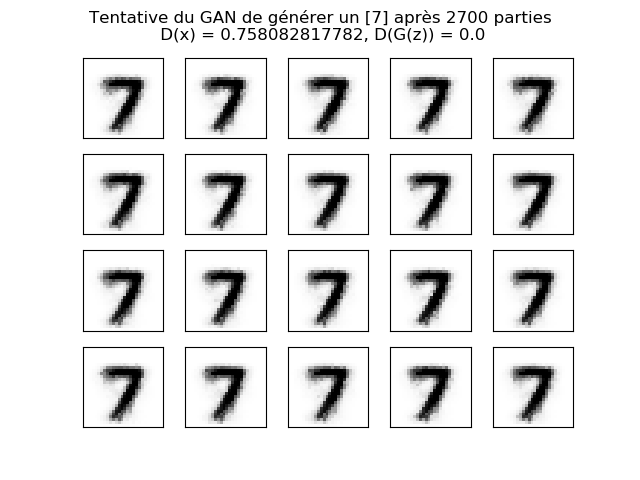
\includegraphics[width=\linewidth]{fig/Wgan_result_1}
    \caption{Résultat du WGAN pour 27 000 parties, D(x) = 7.58)}
    \label{fig:Wgan_result_1_nombres}
\end{subfigure}
\quad
\begin{subfigure}[b]{.6\linewidth}
  \centering
    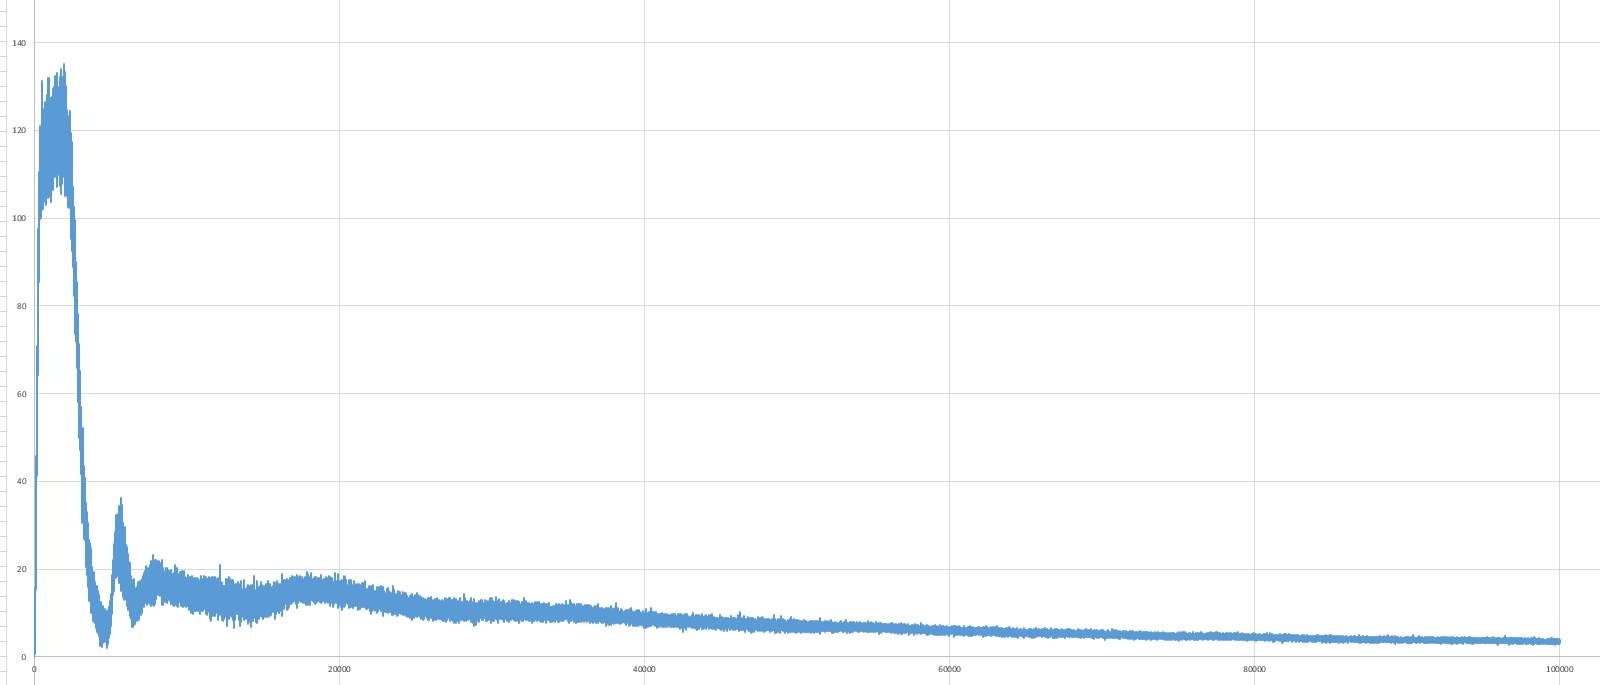
\includegraphics[width=10cm]{fig/Wgan_result_1_courbe}
    \caption{Distance de Wasserstein pendant l'apprentissage}
    \label{fig:Wgan_result_1_courbe}
    \end{subfigure}
    \caption{Apprentissage d'un 7 sans bruit en sortie (100 000 parties)}
    \label{fig:Wgan_result_1}
\end{figure}
	La figure \ref{fig:Wgan_result_1_nombres} montre le résultat de la structure précédente. La première conclusion est que l'algorithme peut fonctionner et donner des résultats, ce qui est très encourageant. On observe que les 7 sont biens formés, que la délimitation avec la partie blanche n'est pas nette, et qu'il ont tous sensiblement la même forme. On est donc dans un mode collapse qui se confirme lorsque l'on regarde l'évolution. Un seul 7 est visible à chaque instant, mais sa forme évolue constamment entre plusieurs 7 différents.\\
	La figure \ref{fig:Wgan_result_1_courbe} montre l'évolution du score au cours de ce même apprentissage. On y observe bien la pertinence entre la distance de Wasserstein (le score si les convergence sont bien faites) et la qualité visuelle des chiffres. \\
	La forte augmentation au début correspond à la phase d'initialisation, où l'on ne fait apprendre que le critique afin de calculer la divergence initiale. On observe au cours de l'apprentissage l'amélioration de l'image de façon synchrone avec la chute du score, avec une très rapide progression au début (pour les contours grossier), puis une progression plus limitée (pour les contours fins), et enfin une stagnation visuelle à partir de 25 000 apprentissages.

	L'étape suivante consiste à tenter d'obtenir de la diversité, soit en s’éloignant du mode Collapse, soit en produisant plusieurs chiffres (objectifs en réalité très similaires). 

	Nous avons introduit du bruit en couche de sortie (comme vu au chapitre 2.7) afin d'observer de la diversité. En tentant de produire plusieurs chiffres, nous n'avons eu aucun résultat concluant, seul une tâche centrale persiste, que l'on peut peut être interpréter comme une moyenne des chiffres existants. Avec un seul chiffre, on obtient le résultat de la figure \ref{fig:Wgan_result_2_nombres}, on parvient donc à sortir du Collapse, mais on perd en qualité visuelle, le tracé n'étant plus lisse, mais fragmenté.

	Attention, ces derniers résultats sont à prendre avec beaucoup de précaution, ils ont été faits rapidement en fin de projet et n'ont donc pas pu être affinés. Ainsi les conclusions sont que le WGAN fonctionne, que les métriques qu'ils proposent semblent pertinentes vis à vis de ce qui est présenté dans le papier, mais qu'il est soumis à une part importante des problèmes des GANs, une intolérance vis à vis des paramètres approximatifs et le mode Collapse.

\begin{figure}[ht!]
  \centering
  	\begin{subfigure}[b]{.4\linewidth}
    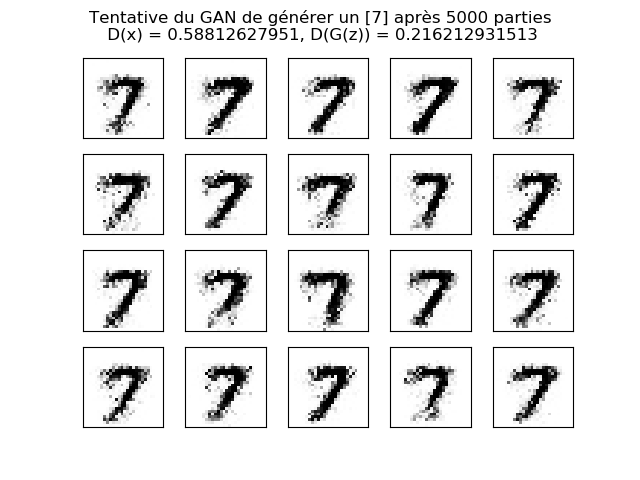
\includegraphics[width=5cm]{fig/Wgan_result_2}
    \caption{Résultat du WGAN pour 50 000 parties, D(x) = 0.58)}
    \label{fig:Wgan_result_2_nombres}
\end{subfigure}
\quad
\begin{subfigure}[b]{.4\linewidth}
  \centering
    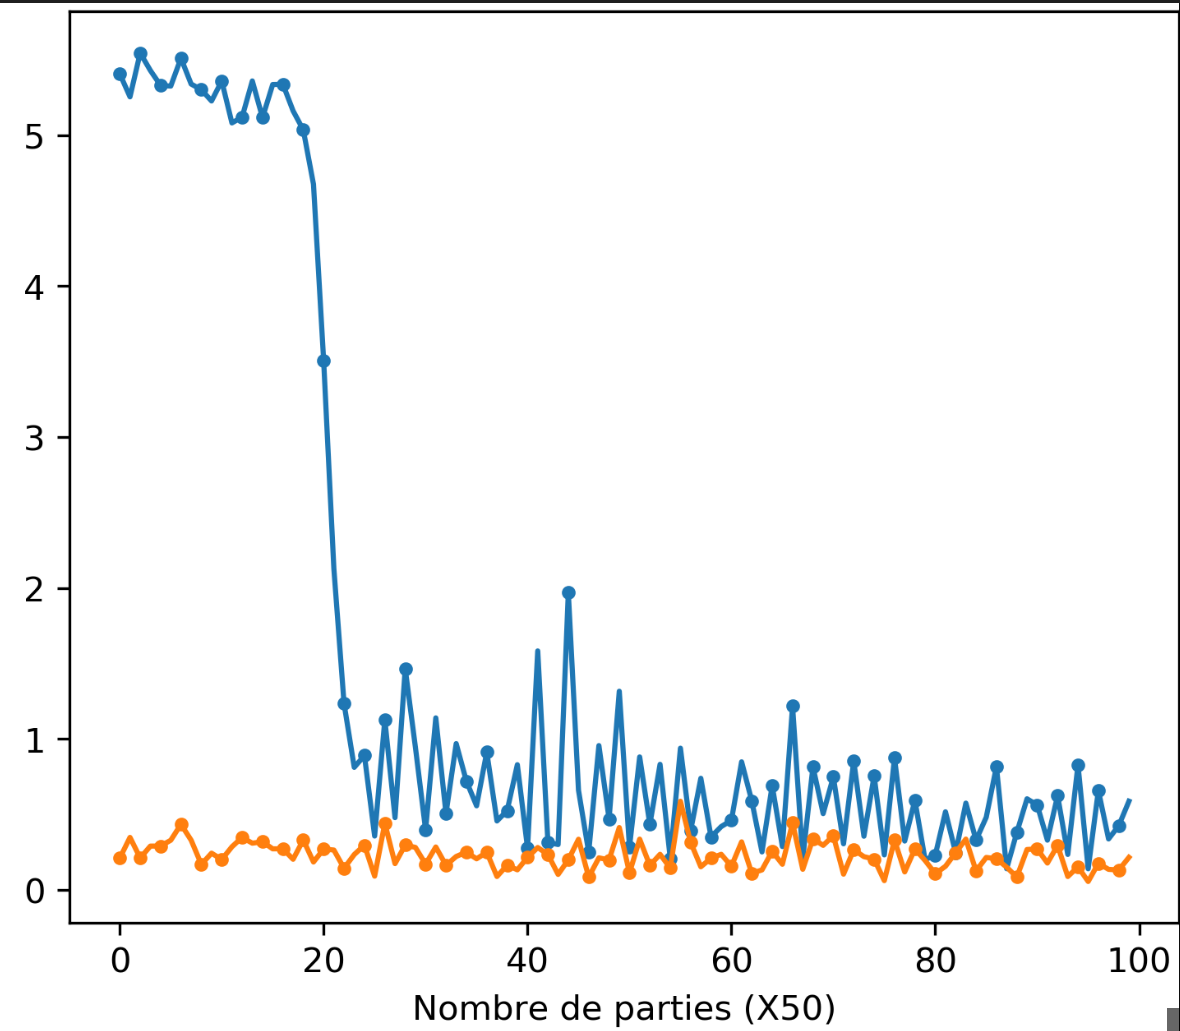
\includegraphics[width=5cm]{fig/Wgan_result_2_courbe}
    \caption{Distance de Wasserstein pendant l'apprentissage}
    \label{fig:Wgan_result_2_courbe}
    \end{subfigure}
    \caption{Apprentissage d'un 7 avec bruit en sortie (100 000 parties)}
    \label{fig:Wgan_result_2}
\end{figure}
 \section{Réflexion sur l'approche}




 \subsection{Utilisation de la distance de Wasserstein pour évaluer un générateur}
 \subsection{Problème du caractère Lipschitziens des réseaux de neurones}
 \subsection{Peut-on adapter la logique de cette algorithme à d'autre méthode ?}